\documentclass[11pt,compress,t,notes=noshow, xcolor=table]{beamer}
\usepackage[]{graphicx}\usepackage[]{color}
% maxwidth is the original width if it is less than linewidth
% otherwise use linewidth (to make sure the graphics do not exceed the margin)
\makeatletter
\def\maxwidth{ %
  \ifdim\Gin@nat@width>\linewidth
    \linewidth
  \else
    \Gin@nat@width
  \fi
}
\makeatother

\definecolor{fgcolor}{rgb}{0.345, 0.345, 0.345}
\newcommand{\hlnum}[1]{\textcolor[rgb]{0.686,0.059,0.569}{#1}}%
\newcommand{\hlstr}[1]{\textcolor[rgb]{0.192,0.494,0.8}{#1}}%
\newcommand{\hlcom}[1]{\textcolor[rgb]{0.678,0.584,0.686}{\textit{#1}}}%
\newcommand{\hlopt}[1]{\textcolor[rgb]{0,0,0}{#1}}%
\newcommand{\hlstd}[1]{\textcolor[rgb]{0.345,0.345,0.345}{#1}}%
\newcommand{\hlkwa}[1]{\textcolor[rgb]{0.161,0.373,0.58}{\textbf{#1}}}%
\newcommand{\hlkwb}[1]{\textcolor[rgb]{0.69,0.353,0.396}{#1}}%
\newcommand{\hlkwc}[1]{\textcolor[rgb]{0.333,0.667,0.333}{#1}}%
\newcommand{\hlkwd}[1]{\textcolor[rgb]{0.737,0.353,0.396}{\textbf{#1}}}%
\let\hlipl\hlkwb

\usepackage{framed}
\makeatletter
\newenvironment{kframe}{%
 \def\at@end@of@kframe{}%
 \ifinner\ifhmode%
  \def\at@end@of@kframe{\end{minipage}}%
  \begin{minipage}{\columnwidth}%
 \fi\fi%
 \def\FrameCommand##1{\hskip\@totalleftmargin \hskip-\fboxsep
 \colorbox{shadecolor}{##1}\hskip-\fboxsep
     % There is no \\@totalrightmargin, so:
     \hskip-\linewidth \hskip-\@totalleftmargin \hskip\columnwidth}%
 \MakeFramed {\advance\hsize-\width
   \@totalleftmargin\z@ \linewidth\hsize
   \@setminipage}}%
 {\par\unskip\endMakeFramed%
 \at@end@of@kframe}
\makeatother

\definecolor{shadecolor}{rgb}{.97, .97, .97}
\definecolor{messagecolor}{rgb}{0, 0, 0}
\definecolor{warningcolor}{rgb}{1, 0, 1}
\definecolor{errorcolor}{rgb}{1, 0, 0}
\newenvironment{knitrout}{}{} % an empty environment to be redefined in TeX

\usepackage{alltt}
\newcommand{\SweaveOpts}[1]{}  % do not interfere with LaTeX
\newcommand{\SweaveInput}[1]{} % because they are not real TeX commands
\newcommand{\Sexpr}[1]{}       % will only be parsed by R



\usepackage[english]{babel}
\usepackage[utf8]{inputenc}

\usepackage{dsfont}
\usepackage{verbatim}
\usepackage{amsmath}
\usepackage{amsfonts}
\usepackage{bm}
\usepackage{csquotes}
\usepackage{multirow}
\usepackage{longtable}
\usepackage{booktabs}
\usepackage{enumerate}
\usepackage[absolute,overlay]{textpos}
\usepackage{psfrag}
\usepackage{algorithm}
\usepackage{algpseudocode}
\usepackage{eqnarray}
\usepackage{arydshln}
\usepackage{tabularx}
\usepackage{placeins}
\usepackage{tikz}
\usepackage{setspace}
\usepackage{colortbl}
\usepackage{mathtools}
\usepackage{wrapfig}
\usepackage{bm}
\usetikzlibrary{shapes,arrows,automata,positioning,calc,chains,trees, shadows}
\tikzset{
  %Define standard arrow tip
  >=stealth',
  %Define style for boxes
  punkt/.style={
    rectangle,
    rounded corners,
    draw=black, very thick,
    text width=6.5em,
    minimum height=2em,
    text centered},
  % Define arrow style
  pil/.style={
    ->,
    thick,
    shorten <=2pt,
    shorten >=2pt,}
}
\usepackage{subfig}


% Defines macros and environments
\usepackage{bbm}
% basic latex stuff
\newcommand{\pkg}[1]{{\fontseries{b}\selectfont #1}} %fontstyle for R packages
\newcommand{\lz}{\vspace{0.5cm}} %vertical space
\newcommand{\dlz}{\vspace{1cm}} %double vertical space
\newcommand{\oneliner}[1] % Oneliner for important statements
{\begin{block}{}\begin{center}\begin{Large}#1\end{Large}\end{center}\end{block}}


%new environments
\newenvironment{vbframe}  %frame with breaks and verbatim
{
 \begin{frame}[containsverbatim,allowframebreaks]
}
{
\end{frame}
}

\newenvironment{vframe}  %frame with verbatim without breaks (to avoid numbering one slided frames)
{
 \begin{frame}[containsverbatim]
}
{
\end{frame}
}

\newenvironment{blocki}[1]   % itemize block
{
 \begin{block}{#1}\begin{itemize}
}
{
\end{itemize}\end{block}
}

\newenvironment{fragileframe}[2]{  %fragile frame with framebreaks
\begin{frame}[allowframebreaks, fragile, environment = fragileframe]
\frametitle{#1}
#2}
{\end{frame}}


\newcommand{\myframe}[2]{  %short for frame with framebreaks
\begin{frame}[allowframebreaks]
\frametitle{#1}
#2
\end{frame}}

\newcommand{\remark}[1]{
  \textbf{Remark:} #1
}

\newcommand{\citebutton}[2]{%
\NoCaseChange{\resizebox{!}{9pt}{\protect\beamergotobutton{\href{#2}{#1}}}}%
}



\newenvironment{deleteframe}
{
\begingroup
\usebackgroundtemplate{\includegraphics[width=\paperwidth,height=\paperheight]{../style/color/red.png}}
 \begin{frame}
}
{
\end{frame}
\endgroup
}
\newenvironment{simplifyframe}
{
\begingroup
\usebackgroundtemplate{\includegraphics[width=\paperwidth,height=\paperheight]{../style/color/yellow.png}}
 \begin{frame}
}
{
\end{frame}
\endgroup
}\newenvironment{draftframe}
{
\begingroup
\usebackgroundtemplate{\includegraphics[width=\paperwidth,height=\paperheight]{../style/color/green.jpg}}
 \begin{frame}
}
{
\end{frame}
\endgroup
}
% https://tex.stackexchange.com/a/261480: textcolor that works in mathmode
\makeatletter
\renewcommand*{\@textcolor}[3]{%
  \protect\leavevmode
  \begingroup
    \color#1{#2}#3%
  \endgroup
}
\makeatother


%\usetheme{lmu-lecture}
\newcommand{\titlefigure}{figure_man/riskmin_bilevel3.png}
\newcommand{\learninggoals}{
\item Definition of HPO objective and components
\item Understand its properties
\item What makes tuning challenging}
\usepackage{../../style/lmu-lecture}

\let\code=\texttt
\let\proglang=\textsf

\setkeys{Gin}{width=0.9\textwidth}

\title{Introduction to Machine Learning}
% \author{Bernd Bischl, Christoph Molnar, Daniel Schalk, Fabian Scheipl}
\institute{\href{https://compstat-lmu.github.io/lecture_i2ml/}{compstat-lmu.github.io/lecture\_i2ml}}
\date{}

\setbeamertemplate{frametitle}{\expandafter\uppercase\expandafter\insertframetitle}



\begin{document}

% Load all R packages and set up knitr

% This file loads R packages, configures knitr options and sets preamble.Rnw as parent file
% IF YOU MODIFY THIS, PLZ ALSO MODIFY setup.Rmd ACCORDINGLY...








% Defines macros and environments
% math spaces
\ifdefined\N                                                                
\renewcommand{\N}{\mathds{N}} % N, naturals
\else \newcommand{\N}{\mathds{N}} \fi 
\newcommand{\Z}{\mathds{Z}} % Z, integers
\newcommand{\Q}{\mathds{Q}} % Q, rationals
\newcommand{\R}{\mathds{R}} % R, reals
\ifdefined\C 
  \renewcommand{\C}{\mathds{C}} % C, complex
\else \newcommand{\C}{\mathds{C}} \fi
\newcommand{\continuous}{\mathcal{C}} % C, space of continuous functions
\newcommand{\M}{\mathcal{M}} % machine numbers
\newcommand{\epsm}{\epsilon_m} % maximum error

% counting / finite sets
\newcommand{\setzo}{\{0, 1\}} % set 0, 1
\newcommand{\setmp}{\{-1, +1\}} % set -1, 1
\newcommand{\unitint}{[0, 1]} % unit interval

% basic math stuff
\newcommand{\xt}{\tilde x} % x tilde
\newcommand{\argmax}{\operatorname{arg\,max}} % argmax
\newcommand{\argmin}{\operatorname{arg\,min}} % argmin
\newcommand{\argminlim}{\mathop{\mathrm{arg\,min}}\limits} % argmax with limits
\newcommand{\argmaxlim}{\mathop{\mathrm{arg\,max}}\limits} % argmin with limits  
\newcommand{\sign}{\operatorname{sign}} % sign, signum
\newcommand{\I}{\mathbb{I}} % I, indicator
\newcommand{\order}{\mathcal{O}} % O, order
\newcommand{\pd}[2]{\frac{\partial{#1}}{\partial #2}} % partial derivative
\newcommand{\floorlr}[1]{\left\lfloor #1 \right\rfloor} % floor
\newcommand{\ceillr}[1]{\left\lceil #1 \right\rceil} % ceiling

% sums and products
\newcommand{\sumin}{\sum\limits_{i=1}^n} % summation from i=1 to n
\newcommand{\sumim}{\sum\limits_{i=1}^m} % summation from i=1 to m
\newcommand{\sumjn}{\sum\limits_{j=1}^n} % summation from j=1 to p
\newcommand{\sumjp}{\sum\limits_{j=1}^p} % summation from j=1 to p
\newcommand{\sumik}{\sum\limits_{i=1}^k} % summation from i=1 to k
\newcommand{\sumkg}{\sum\limits_{k=1}^g} % summation from k=1 to g
\newcommand{\sumjg}{\sum\limits_{j=1}^g} % summation from j=1 to g
\newcommand{\meanin}{\frac{1}{n} \sum\limits_{i=1}^n} % mean from i=1 to n
\newcommand{\meanim}{\frac{1}{m} \sum\limits_{i=1}^m} % mean from i=1 to n
\newcommand{\meankg}{\frac{1}{g} \sum\limits_{k=1}^g} % mean from k=1 to g
\newcommand{\prodin}{\prod\limits_{i=1}^n} % product from i=1 to n
\newcommand{\prodkg}{\prod\limits_{k=1}^g} % product from k=1 to g
\newcommand{\prodjp}{\prod\limits_{j=1}^p} % product from j=1 to p

% linear algebra
\newcommand{\one}{\boldsymbol{1}} % 1, unitvector
\newcommand{\zero}{\mathbf{0}} % 0-vector
\newcommand{\id}{\boldsymbol{I}} % I, identity
\newcommand{\diag}{\operatorname{diag}} % diag, diagonal
\newcommand{\trace}{\operatorname{tr}} % tr, trace
\newcommand{\spn}{\operatorname{span}} % span
\newcommand{\scp}[2]{\left\langle #1, #2 \right\rangle} % <.,.>, scalarproduct
\newcommand{\mat}[1]{\begin{pmatrix} #1 \end{pmatrix}} % short pmatrix command
\newcommand{\Amat}{\mathbf{A}} % matrix A
\newcommand{\Deltab}{\mathbf{\Delta}} % error term for vectors

% basic probability + stats
\renewcommand{\P}{\mathds{P}} % P, probability
\newcommand{\E}{\mathds{E}} % E, expectation
\newcommand{\var}{\mathsf{Var}} % Var, variance
\newcommand{\cov}{\mathsf{Cov}} % Cov, covariance
\newcommand{\corr}{\mathsf{Corr}} % Corr, correlation
\newcommand{\normal}{\mathcal{N}} % N of the normal distribution
\newcommand{\iid}{\overset{i.i.d}{\sim}} % dist with i.i.d superscript
\newcommand{\distas}[1]{\overset{#1}{\sim}} % ... is distributed as ...

% machine learning
\newcommand{\Xspace}{\mathcal{X}} % X, input space
\newcommand{\Yspace}{\mathcal{Y}} % Y, output space
\newcommand{\nset}{\{1, \ldots, n\}} % set from 1 to n
\newcommand{\pset}{\{1, \ldots, p\}} % set from 1 to p
\newcommand{\gset}{\{1, \ldots, g\}} % set from 1 to g
\newcommand{\Pxy}{\mathbb{P}_{xy}} % P_xy
\newcommand{\Exy}{\mathbb{E}_{xy}} % E_xy: Expectation over random variables xy
\newcommand{\xv}{\mathbf{x}} % vector x (bold)
\newcommand{\xtil}{\tilde{\mathbf{x}}} % vector x-tilde (bold)
\newcommand{\yv}{\mathbf{y}} % vector y (bold)
\newcommand{\xy}{(\xv, y)} % observation (x, y)
\newcommand{\xvec}{\left(x_1, \ldots, x_p\right)^\top} % (x1, ..., xp) 
\newcommand{\Xmat}{\mathbf{X}} % Design matrix
\newcommand{\allDatasets}{\mathds{D}} % The set of all datasets
\newcommand{\allDatasetsn}{\mathds{D}_n}  % The set of all datasets of size n 
\newcommand{\D}{\mathcal{D}} % D, data
\newcommand{\Dn}{\D_n} % D_n, data of size n
\newcommand{\Dtrain}{\mathcal{D}_{\text{train}}} % D_train, training set
\newcommand{\Dtest}{\mathcal{D}_{\text{test}}} % D_test, test set
\newcommand{\xyi}[1][i]{\left(\xv^{(#1)}, y^{(#1)}\right)} % (x^i, y^i), i-th observation
\newcommand{\Dset}{\left( \xyi[1], \ldots, \xyi[n]\right)} % {(x1,y1)), ..., (xn,yn)}, data
\newcommand{\defAllDatasetsn}{(\Xspace \times \Yspace)^n} % Def. of the set of all datasets of size n 
\newcommand{\defAllDatasets}{\bigcup_{n \in \N}(\Xspace \times \Yspace)^n} % Def. of the set of all datasets 
\newcommand{\xdat}{\left\{ \xv^{(1)}, \ldots, \xv^{(n)}\right\}} % {x1, ..., xn}, input data
\newcommand{\yvec}{\left(y^{(1)}, \hdots, y^{(n)}\right)^\top} % (y1, ..., yn), vector of outcomes
\renewcommand{\xi}[1][i]{\xv^{(#1)}} % x^i, i-th observed value of x
\newcommand{\yi}[1][i]{y^{(#1)}} % y^i, i-th observed value of y 
\newcommand{\xivec}{\left(x^{(i)}_1, \ldots, x^{(i)}_p\right)^\top} % (x1^i, ..., xp^i), i-th observation vector
\newcommand{\xj}{\xv_j} % x_j, j-th feature
\newcommand{\xjvec}{\left(x^{(1)}_j, \ldots, x^{(n)}_j\right)^\top} % (x^1_j, ..., x^n_j), j-th feature vector
\newcommand{\phiv}{\mathbf{\phi}} % Basis transformation function phi
\newcommand{\phixi}{\mathbf{\phi}^{(i)}} % Basis transformation of xi: phi^i := phi(xi)

%%%%%% ml - models general
\newcommand{\lamv}{\bm{\lambda}} % lambda vector, hyperconfiguration vector
\newcommand{\Lam}{\bm{\Lambda}}	 % Lambda, space of all hpos
% Inducer / Inducing algorithm
\newcommand{\preimageInducer}{\left(\defAllDatasets\right)\times\Lam} % Set of all datasets times the hyperparameter space
\newcommand{\preimageInducerShort}{\allDatasets\times\Lam} % Set of all datasets times the hyperparameter space
% Inducer / Inducing algorithm
\newcommand{\ind}{\mathcal{I}} % Inducer, inducing algorithm, learning algorithm 

% continuous prediction function f
\newcommand{\ftrue}{f_{\text{true}}}  % True underlying function (if a statistical model is assumed)
\newcommand{\ftruex}{\ftrue(\xv)} % True underlying function (if a statistical model is assumed)
\newcommand{\fx}{f(\xv)} % f(x), continuous prediction function
\newcommand{\fdomains}{f: \Xspace \rightarrow \R^g} % f with domain and co-domain
\newcommand{\Hspace}{\mathcal{H}} % hypothesis space where f is from
\newcommand{\fbayes}{f^{\ast}} % Bayes-optimal model
\newcommand{\fxbayes}{f^{\ast}(\xv)} % Bayes-optimal model
\newcommand{\fkx}[1][k]{f_{#1}(\xv)} % f_j(x), discriminant component function
\newcommand{\fh}{\hat{f}} % f hat, estimated prediction function
\newcommand{\fxh}{\fh(\xv)} % fhat(x)
\newcommand{\fxt}{f(\xv ~|~ \thetab)} % f(x | theta)
\newcommand{\fxi}{f\left(\xv^{(i)}\right)} % f(x^(i))
\newcommand{\fxih}{\hat{f}\left(\xv^{(i)}\right)} % f(x^(i))
\newcommand{\fxit}{f\left(\xv^{(i)} ~|~ \thetab\right)} % f(x^(i) | theta)
\newcommand{\fhD}{\fh_{\D}} % fhat_D, estimate of f based on D
\newcommand{\fhDtrain}{\fh_{\Dtrain}} % fhat_Dtrain, estimate of f based on D
\newcommand{\fhDnlam}{\fh_{\Dn, \lamv}} %model learned on Dn with hp lambda
\newcommand{\fhDlam}{\fh_{\D, \lamv}} %model learned on D with hp lambda
\newcommand{\fhDnlams}{\fh_{\Dn, \lamv^\ast}} %model learned on Dn with optimal hp lambda 
\newcommand{\fhDlams}{\fh_{\D, \lamv^\ast}} %model learned on D with optimal hp lambda 

% discrete prediction function h
\newcommand{\hx}{h(\xv)} % h(x), discrete prediction function
\newcommand{\hh}{\hat{h}} % h hat
\newcommand{\hxh}{\hat{h}(\xv)} % hhat(x)
\newcommand{\hxt}{h(\xv | \thetab)} % h(x | theta)
\newcommand{\hxi}{h\left(\xi\right)} % h(x^(i))
\newcommand{\hxit}{h\left(\xi ~|~ \thetab\right)} % h(x^(i) | theta)
\newcommand{\hbayes}{h^{\ast}} % Bayes-optimal classification model
\newcommand{\hxbayes}{h^{\ast}(\xv)} % Bayes-optimal classification model

% yhat
\newcommand{\yh}{\hat{y}} % yhat for prediction of target
\newcommand{\yih}{\hat{y}^{(i)}} % yhat^(i) for prediction of ith targiet
\newcommand{\resi}{\yi- \yih}

% theta
\newcommand{\thetah}{\hat{\theta}} % theta hat
\newcommand{\thetab}{\bm{\theta}} % theta vector
\newcommand{\thetabh}{\bm{\hat\theta}} % theta vector hat
\newcommand{\thetat}[1][t]{\thetab^{[#1]}} % theta^[t] in optimization
\newcommand{\thetatn}[1][t]{\thetab^{[#1 +1]}} % theta^[t+1] in optimization
\newcommand{\thetahDnlam}{\thetabh_{\Dn, \lamv}} %theta learned on Dn with hp lambda
\newcommand{\thetahDlam}{\thetabh_{\D, \lamv}} %theta learned on D with hp lambda
\newcommand{\mint}{\min_{\thetab \in \Theta}} % min problem theta
\newcommand{\argmint}{\argmin_{\thetab \in \Theta}} % argmin theta

% densities + probabilities
% pdf of x 
\newcommand{\pdf}{p} % p
\newcommand{\pdfx}{p(\xv)} % p(x)
\newcommand{\pixt}{\pi(\xv~|~ \thetab)} % pi(x|theta), pdf of x given theta
\newcommand{\pixit}{\pi\left(\xi ~|~ \thetab\right)} % pi(x^i|theta), pdf of x given theta
\newcommand{\pixii}{\pi\left(\xi\right)} % pi(x^i), pdf of i-th x 

% pdf of (x, y)
\newcommand{\pdfxy}{p(\xv,y)} % p(x, y)
\newcommand{\pdfxyt}{p(\xv, y ~|~ \thetab)} % p(x, y | theta)
\newcommand{\pdfxyit}{p\left(\xi, \yi ~|~ \thetab\right)} % p(x^(i), y^(i) | theta)

% pdf of x given y
\newcommand{\pdfxyk}[1][k]{p(\xv | y= #1)} % p(x | y = k)
\newcommand{\lpdfxyk}[1][k]{\log p(\xv | y= #1)} % log p(x | y = k)
\newcommand{\pdfxiyk}[1][k]{p\left(\xi | y= #1 \right)} % p(x^i | y = k)

% prior probabilities
\newcommand{\pik}[1][k]{\pi_{#1}} % pi_k, prior
\newcommand{\lpik}[1][k]{\log \pi_{#1}} % log pi_k, log of the prior
\newcommand{\pit}{\pi(\thetab)} % Prior probability of parameter theta

% posterior probabilities
\newcommand{\post}{\P(y = 1 ~|~ \xv)} % P(y = 1 | x), post. prob for y=1
\newcommand{\postk}[1][k]{\P(y = #1 ~|~ \xv)} % P(y = k | y), post. prob for y=k
\newcommand{\pidomains}{\pi: \Xspace \rightarrow \unitint} % pi with domain and co-domain
\newcommand{\pibayes}{\pi^{\ast}} % Bayes-optimal classification model
\newcommand{\pixbayes}{\pi^{\ast}(\xv)} % Bayes-optimal classification model
\newcommand{\pix}{\pi(\xv)} % pi(x), P(y = 1 | x)
\newcommand{\pikx}[1][k]{\pi_{#1}(\xv)} % pi_k(x), P(y = k | x)
\newcommand{\pikxt}[1][k]{\pi_{#1}(\xv ~|~ \thetab)} % pi_k(x | theta), P(y = k | x, theta)
\newcommand{\pixh}{\hat \pi(\xv)} % pi(x) hat, P(y = 1 | x) hat
\newcommand{\pikxh}[1][k]{\hat \pi_{#1}(\xv)} % pi_k(x) hat, P(y = k | x) hat
\newcommand{\pixih}{\hat \pi(\xi)} % pi(x^(i)) with hat
\newcommand{\pikxih}[1][k]{\hat \pi_{#1}(\xi)} % pi_k(x^(i)) with hat
\newcommand{\pdfygxt}{p(y ~|~\xv, \thetab)} % p(y | x, theta)
\newcommand{\pdfyigxit}{p\left(\yi ~|~\xi, \thetab\right)} % p(y^i |x^i, theta)
\newcommand{\lpdfygxt}{\log \pdfygxt } % log p(y | x, theta)
\newcommand{\lpdfyigxit}{\log \pdfyigxit} % log p(y^i |x^i, theta)

% probababilistic
\newcommand{\bayesrulek}[1][k]{\frac{\P(\xv | y= #1) \P(y= #1)}{\P(\xv)}} % Bayes rule
\newcommand{\muk}{\bm{\mu_k}} % mean vector of class-k Gaussian (discr analysis) 

% residual and margin
\newcommand{\eps}{\epsilon} % residual, stochastic
\newcommand{\epsi}{\epsilon^{(i)}} % epsilon^i, residual, stochastic
\newcommand{\epsh}{\hat{\epsilon}} % residual, estimated
\newcommand{\yf}{y \fx} % y f(x), margin
\newcommand{\yfi}{\yi \fxi} % y^i f(x^i), margin
\newcommand{\Sigmah}{\hat \Sigma} % estimated covariance matrix
\newcommand{\Sigmahj}{\hat \Sigma_j} % estimated covariance matrix for the j-th class

% ml - loss, risk, likelihood
\newcommand{\Lyf}{L\left(y, f\right)} % L(y, f), loss function
\newcommand{\Lxy}{L\left(y, \fx\right)} % L(y, f(x)), loss function
\newcommand{\Lxyi}{L\left(\yi, \fxi\right)} % loss of observation
\newcommand{\Lxyt}{L\left(y, \fxt\right)} % loss with f parameterized
\newcommand{\Lxyit}{L\left(\yi, \fxit\right)} % loss of observation with f parameterized
\newcommand{\Lxym}{L\left(\yi, f\left(\bm{\tilde{x}}^{(i)} ~|~ \thetab\right)\right)} % loss of observation with f parameterized
\newcommand{\Lpixy}{L\left(y, \pix\right)} % loss in classification
\newcommand{\Lpixyi}{L\left(\yi, \pixii\right)} % loss of observation in classification
\newcommand{\Lpixyt}{L\left(y, \pixt\right)} % loss with pi parameterized
\newcommand{\Lpixyit}{L\left(\yi, \pixit\right)} % loss of observation with pi parameterized
\newcommand{\Lhxy}{L\left(y, \hx\right)} % L(y, h(x)), loss function on discrete classes
\newcommand{\Lr}{L\left(r\right)} % L(r), loss defined on residual (reg) / margin (classif)
\newcommand{\lone}{|y - \fx|} % L1 loss
\newcommand{\ltwo}{\left(y - \fx\right)^2} % L2 loss
\newcommand{\lbernoullimp}{\ln(1 + \exp(-y \cdot \fx))} % Bernoulli loss for -1, +1 encoding
\newcommand{\lbernoullizo}{- y \cdot \fx + \log(1 + \exp(\fx))} % Bernoulli loss for 0, 1 encoding
\newcommand{\lcrossent}{- y \log \left(\pix\right) - (1 - y) \log \left(1 - \pix\right)} % cross-entropy loss
\newcommand{\lbrier}{\left(\pix - y \right)^2} % Brier score
\newcommand{\risk}{\mathcal{R}} % R, risk
\newcommand{\riskbayes}{\mathcal{R}^\ast}
\newcommand{\riskf}{\risk(f)} % R(f), risk
\newcommand{\riskdef}{\E_{y|\xv}\left(\Lxy \right)} % risk def (expected loss)
\newcommand{\riskt}{\mathcal{R}(\thetab)} % R(theta), risk
\newcommand{\riske}{\mathcal{R}_{\text{emp}}} % R_emp, empirical risk w/o factor 1 / n
\newcommand{\riskeb}{\bar{\mathcal{R}}_{\text{emp}}} % R_emp, empirical risk w/ factor 1 / n
\newcommand{\riskef}{\riske(f)} % R_emp(f)
\newcommand{\risket}{\mathcal{R}_{\text{emp}}(\thetab)} % R_emp(theta)
\newcommand{\riskr}{\mathcal{R}_{\text{reg}}} % R_reg, regularized risk
\newcommand{\riskrt}{\mathcal{R}_{\text{reg}}(\thetab)} % R_reg(theta)
\newcommand{\riskrf}{\riskr(f)} % R_reg(f)
\newcommand{\riskrth}{\hat{\mathcal{R}}_{\text{reg}}(\thetab)} % hat R_reg(theta)
\newcommand{\risketh}{\hat{\mathcal{R}}_{\text{emp}}(\thetab)} % hat R_emp(theta)
\newcommand{\LL}{\mathcal{L}} % L, likelihood
\newcommand{\LLt}{\mathcal{L}(\thetab)} % L(theta), likelihood
\newcommand{\LLtx}{\mathcal{L}(\thetab | \xv)} % L(theta|x), likelihood
\newcommand{\logl}{\ell} % l, log-likelihood
\newcommand{\loglt}{\logl(\thetab)} % l(theta), log-likelihood
\newcommand{\logltx}{\logl(\thetab | \xv)} % l(theta|x), log-likelihood
\newcommand{\errtrain}{\text{err}_{\text{train}}} % training error
\newcommand{\errtest}{\text{err}_{\text{test}}} % test error
\newcommand{\errexp}{\overline{\text{err}_{\text{test}}}} % avg training error

% lm
\newcommand{\thx}{\thetab^\top \xv} % linear model
\newcommand{\olsest}{(\Xmat^\top \Xmat)^{-1} \Xmat^\top \yv} % OLS estimator in LM 

% resampling
\newcommand{\ntest}{n_{\mathrm{test}}} % size of the test set
\newcommand{\ntrain}{n_{\mathrm{train}}} % size of the train set
\newcommand{\ntesti}[1][i]{n_{\mathrm{test},#1}} % size of the i-th test set
\newcommand{\ntraini}[1][i]{n_{\mathrm{train},#1}} % size of the i-th train set
\newcommand{\Jtrain}{J_\mathrm{train}} % index vector train data
\newcommand{\Jtest}{J_\mathrm{test}} % index vector test data
\newcommand{\Jtraini}[1][i]{J_{\mathrm{train},#1}} % index vector i-th train dataset
\newcommand{\Jtesti}[1][i]{J_{\mathrm{test},#1}} % index vector i-th test dataset
\newcommand{\Dtraini}[1][i]{\mathcal{D}_{\text{train},#1}} % D_train,i, i-th training set
\newcommand{\Dtesti}[1][i]{\mathcal{D}_{\text{test},#1}} % D_test,i, i-th test set

\newcommand{\JSpace}[1][m]{\nset^{#1}} % space of train indices of size n_train
\newcommand{\JtrainSpace}{\nset^{\ntrain}} % space of train indices of size n_train
\newcommand{\JtestSpace}{\nset^{\ntest}} % space of train indices of size n_test
\newcommand{\yJ}[1][J]{\yv_{#1}} % output vector associated to index J
\newcommand{\yJDef}{\left(y^{(J^{(1)})},\dots,y^{(J^{(m)})}\right)} % def of the output vector associated to index J
\newcommand{\JJ}{\mathcal{J}} % cali-J, set of all splits
\newcommand{\JJset}{\left((\Jtraini[1], \Jtesti[1]),\dots,(\Jtraini[B], \Jtesti[B])\right)} % (Jtrain_1,Jtest_1) ...(Jtrain_B,Jtest_B)
\newcommand{\Itrainlam}{\ind(\Dtrain, \lamv)}
% Generalization error
\newcommand{\GE}{\mathrm{GE}} % GE
\newcommand{\GEh}{\widehat{\GE}} % GE-hat 
\newcommand{\GEfull}[1][\ntrain]{\GE(\ind, \lamv, #1, \rho)} % GE full
\newcommand{\GEhholdout}{\GEh_{\Jtrain, \Jtest}(\ind, \lamv, |\Jtrain|, \rho)} % GE hat holdout
\newcommand{\GEhholdouti}[1][i]{\GEh_{\Jtraini[#1], \Jtesti[#1]}(\ind, \lamv, |\Jtraini[#1]|, \rho)} % GE hat holdout i-th set
\newcommand{\GEhlam}{\GEh(\lamv)} % GE-hat(lam) 
\newcommand{\GEhlamsubIJrho}{\GEh_{\ind, \JJ, \rho}(\lamv)} % GE-hat_I,J,rho(lam) 
\newcommand{\GEhresa}{\GEh(\ind, \JJ, \rho, \lamv)} % GE-hat_I,J,rho(lam) 
\newcommand{\GErhoDef}{\lim_{\ntest\rightarrow\infty} \E_{\Dtrain,\Dtest \sim \Pxy} \left[ \rho\left(\yv_{\Jtest}, \FJtestftrain\right)\right]} % GE formal def
\newcommand{\agr}{\mathrm{agr}} % aggregate function
\newcommand{\GEf}{\GE\left(\fh\right)} % GE of a fitted model
\newcommand{\GEfh}{\GEh\left(\fh\right)} % GEh of a fitted model
\newcommand{\GEfL}{\GE\left(\fh, L\right)} % GE of a fitted model wrt loss L
\newcommand{\Lyfhx}{L\left(y, \hat{f}(\xv)\right)} % pointwise loss of fitted model
\newcommand{\GEnf}[1]{GE_n\left(\fh_{#1}\right)} % GE of a fitted model
\newcommand{\GEind}{GE_n\left(\ind_{L, O}\right)} % GE of inducer
\newcommand{\GED}{\GE_{\D}} % GE indexed with data
\newcommand{\EGEn}{EGE_n} % expected GE
\newcommand{\EDn}{\E_{|D| = n}} % expectation wrt data of size n

% performance measure
\newcommand{\rhoL}{\rho_L} % perf. measure derived from pointwise loss
\newcommand{\F}{\boldsymbol{F}} % matrix of prediction scores
\newcommand{\Fi}[1][i]{\F^{(#1)}} % i-th row vector of the predscore mat
\newcommand{\FJ}[1][J]{\F_{#1}} % predscore mat idxvec J 
\newcommand{\FJf}{\FJ[J,f]} % predscore mat idxvec J and model f
\newcommand{\FJtestfh}{\FJ[\Jtest, \fh]} % predscore mat idxvec Jtest and model f hat
\newcommand{\FJtestftrain}{\F_{\Jtest, \Itrainlam}} % predscore mat idxvec Jtest and model f
\newcommand{\FJtestftraini}[1][i]{\F_{\Jtesti[#1],\ind(\Dtraini[#1], \lamv)}}  % predscore mat i-th idxvec Jtest and model f
\newcommand{\FJfDef}{\left(f(\xv^{(J^{(1)})}),\dots, f(\xv^{(J^{(m)})})\right)} % def of predscore mat idxvec J and model f
\newcommand{\preimageRho}{\bigcup_{m\in\N}\left(\Yspace^m\times\R^{m\times g}\right)} % Set of all datasets times HP space

% ml - ROC
\newcommand{\np}{n_{+}} % no. of positive instances
\newcommand{\nn}{n_{-}} % no. of negative instances
\newcommand{\rn}{\pi_{-}} % proportion negative instances
\newcommand{\rp}{\pi_{+}} % proportion negative instances
  % true/false pos/neg:
\newcommand{\tp}{\# \text{TP}} % true pos
\newcommand{\fap}{\# \text{FP}} % false pos (fp taken for partial derivs)
\newcommand{\tn}{\# \text{TN}} % true neg
\newcommand{\fan}{\# \text{FN}} % false neg
%%% HPO Basics 
\newcommand{\Ilam}{\ind_{\lamv}} % inducer with HP
\newcommand{\LamS}{\tilde\Lam} % search space
\newcommand{\lami}[1][i]{\lamv^{(#1)}} % lambda i
\newcommand{\clam}{c(\lamv)} % c(lambda)
\newcommand{\clamh}{c(\lamh)} % c(lambda-hat)
\newcommand{\lams}{\lamv^{*}} % theoretical min of c
\newcommand{\lamh}{\hat{\lamv}} % returned lambda of HPO
\newcommand{\lamp}{\lamv^+} % proposed lambda
\newcommand{\clamp}{c(\lamp)} % c of proposed lambda
\newcommand{\archive}{\mathcal{A}} % archive
\newcommand{\archivet}[1][t]{\mathcal{A}^{[#1]}} % archive at time step t

\newcommand{\tuner}{\mathcal{T}} % tuner
\newcommand{\tunerfull}{\tuner_{\ind,\LamS, \rho,\JJ}} % tuner with inducer, search space, perf measure, resampling strategy

%%% Bayesian Opt
\newcommand{\chlam}{\hat{c}(\lamv)} % post mean of SM 
\newcommand{\shlam}{\hat{\sigma}(\lamv)} % post sd of SM
\newcommand{\vhlam}{\hat{\sigma}^2(\lamv)} % post var of SM
\newcommand{\ulam}{u(\lamv)} % acquisition function
\newcommand{\lambdaopt}{\lambda^{*}} % minimum of the black box function Psi
\newcommand{\metadata}{\left\{\left(\lami, \Psi^{[i]}\right)\right\}} % metadata for the Gaussian process
\newcommand{\lamvec}{\left(\lambda^{[1]}, \dots, \lambda^{[\minit]}\right)} % vector of different inputs
\newcommand{\minit}{m_{\text{init}}} % size of the initial design

%%% Multifidelity / Hyperband
\newcommand{\lambu}{\lambda_{\text{budget}}} % single lambda_budget component HP
\newcommand{\lamfid}{\lambda_{\text{fid}}} % single lambda fidelity
\newcommand{\lamfidl}{\lamfid^{\textrm{low}}} % single lambda fidelity lower
\newcommand{\lamfidu}{\lamfid^{\textrm{upp}}} % single lambda fidelity upper
\newcommand{\etahb}{\eta_{\text{HB}}}  % HB multiplier eta

%! includes: tuning-intro
\lecturechapter{Hyperparameter Tuning - Problem Definition }
\lecture{Introduction to Machine Learning}
\sloppy


\begin{vbframe}{Hyperparameter Optimization}

\vskip 3em
\textbf{Hyperparameters (HP)} $\lamv$ are parameters that are \emph{inputs} to learner $\ind$ which performs ERM on training data set to find optimal \textbf{model parameters} $\thetab$. 
HPs can influence the generalization performance in a non-trivial and subtle way. 

\vskip 2em

\textbf{Hyperparameter optimization (HPO) / Tuning} is the process of finding a well-performing hyperparameter configuration (HPC) $\lamv \in \LamS$ for an learner $\Ilam$. 
\end{vbframe}

% \begin{vbframe}{Hyperparameter Tuning}
% \begin{itemize}
% \item Optimize hyperparameters for learner w.r.t. prediction error
% Tuner proposes configuration, eval by resampling, tuner receives performance, iterate
% \end{itemize}
% \begin{columns}[c, onlytextwidth]
% \column{0.45\textwidth}
% FIGURE SOURCE: No source
  % 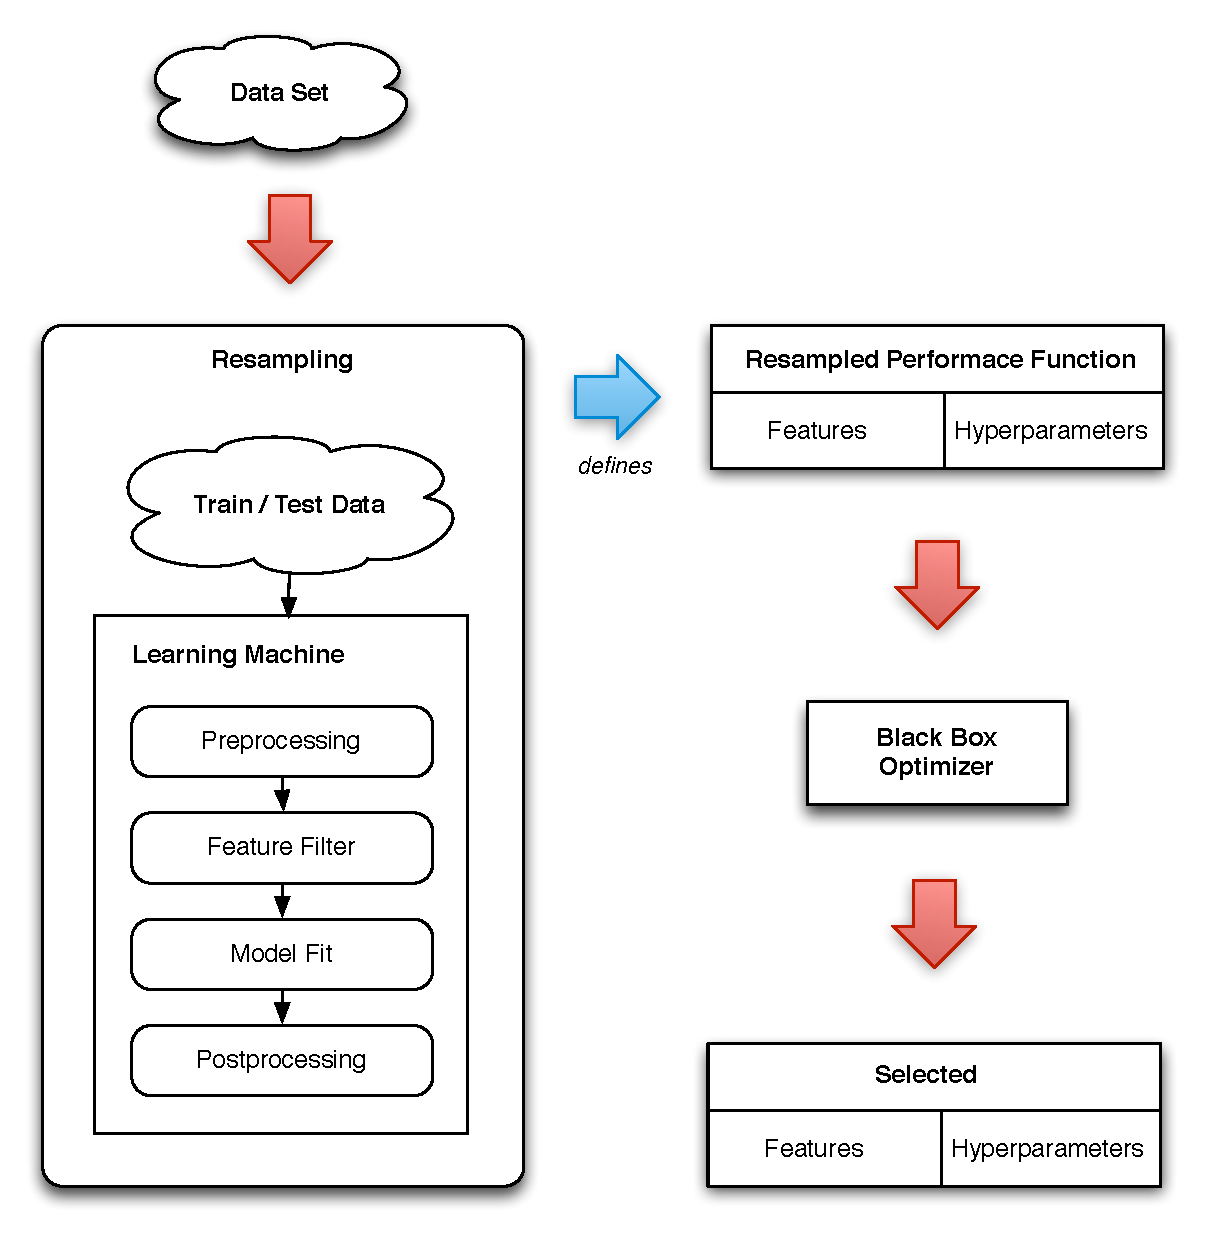
\includegraphics[trim={0cm 0cm 0cm 0cm}, clip, width=1.2\textwidth]{figure_man/chain.jpg}
% \column{0.45\textwidth}
  % FIGURE SOURCE: https://drive.google.com/open?id=1wY3aUZxIMZPje3vR0t2yWiDMx_osXRCi
% 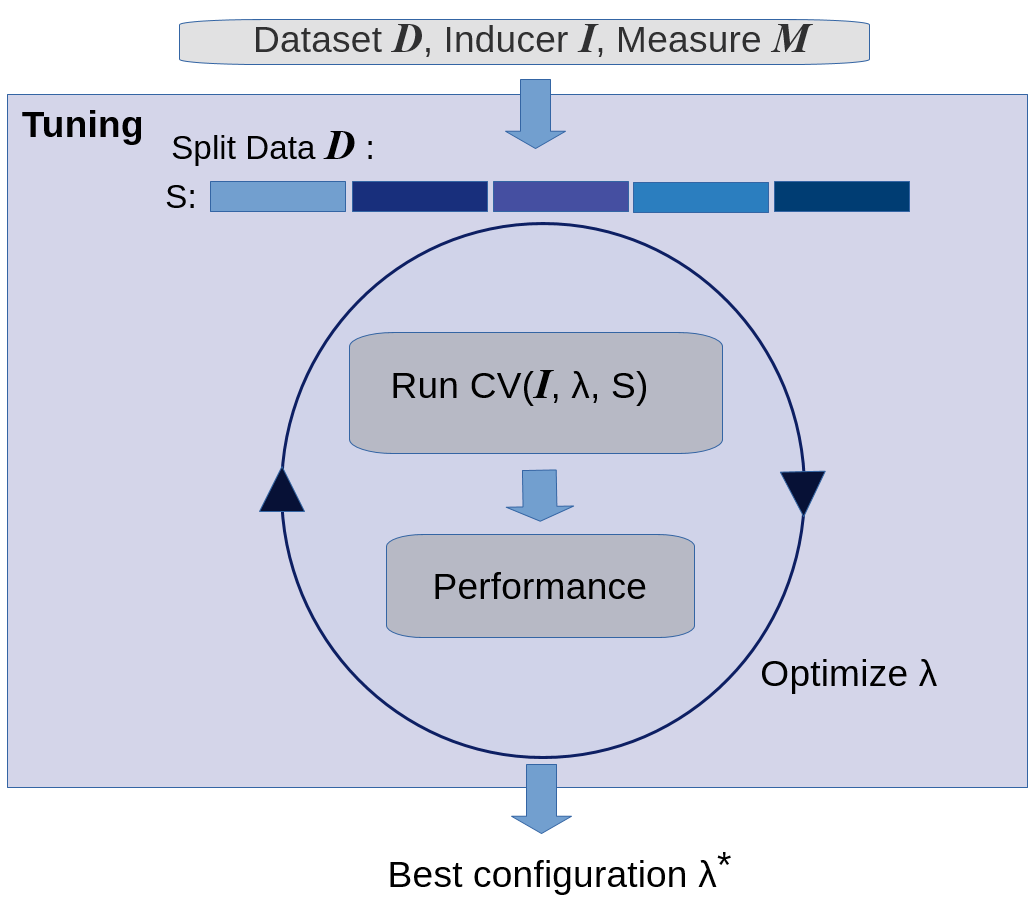
\includegraphics[trim={1cm 0cm 1cm 0cm}, clip, width=1.2\textwidth]{figure_man/tuning_process.jpg}
% \end{columns}

% \end{vbframe}

% \framebreak
\begin{vbframe}{Objective and Search Space}
% \begin{itemize}
% \item HPO  algorithms  automatically identify  a  well-performing  hyperparameter configuration (HPC) $\lamv \in \LamS$ for an learner $\Ilam$. 
Search space $\LamS \subset \Lam$ with all optimized HPs and ranges:
$$\LamS = \LamS_1 \times \LamS_2 \times \dots \times \LamS_l$$
 where $\LamS_i$ is a bounded subset of the domain of the i-th HP $\Lam_i$, and can be either continuous, discrete, or categorical. 
% \end{itemize}

% \framebreak
% \begin{footnotesize}

\vspace{1cm}

The general HPO problem is defined as:
\begin{eqnarray*}
    \lams \in \argmin_{\lamv \in \LamS} \clam = \argmin_{\lamv \in \LamS} 
    %\GEhlamsubIJrho
    \GEhresa
\end{eqnarray*}
with $\lams$ as theoretical optimum, and $\clam$ is short for estim. gen. error
when $\ind$, resampling splits $\JJ$, performance measure $\rho$ are fixed.
\end{vbframe}

% \begin{vbframe}{Objective and Search Space}
% \begin{itemize}
% \item The data set $\D$
% \item A learner $\Ilam$ (possibly: several competing learners?) to be tuned %(e.g. a decision tree classifier)
% \item The learner's hyperparameters and their respective regions-of-interest $\LamS$ over which we optimize % (e.g. $\texttt{tree depth} \in \{1, 2, ..., 20\}$)
% \item The performance measure $\rho$, as determined by the application.\\ Not necessarily identical to the loss function that defines the risk minimization problem for the learner!\\ 
% % We could even be interested in multiple measures simultaneously, e.g., accuracy and computation time of our model, TPR and PPV, etc. 
% \item A (resampling) procedure for estimating the predictive performance which gives rise to the splits $\JJ$
%    % The expected performance on unseen data can be estimated by holdout (i.e., a single train-test-split) or more advanced techniques like cross-validation.
% % More on this later.
% \end{itemize}
% \end{vbframe}

\begin{vbframe}{Objective and Search Space}
\begin{eqnarray*}
    \lams \in \argmin_{\lamv \in \LamS} \clam = \argmin_{\lamv \in \LamS} 
    %\GEhlamsubIJrho
    \GEhresa
\end{eqnarray*}
\begin{figure}[h]
    \centering
    \includegraphics[width = 0.65\textwidth]{figure/hpo_loop_1.eps}
    %{figures/riskmin_bilevel3.png}
\end{figure}

\begin{itemize}
    \item Evals are stored in \textbf{archive} $\archive = ((\lamv^{(1)}, c(\lamv^{(1)})), (\lamv^{(2)}, c(\lamv^{(2)})), \dots)$, with $\archivet[t+1] = \archivet[t] \cup (\lamp, \clamp)$.
% \end{footnotesize}

% \medskip

 \item We can define tuner as function $\tau: (\D, \ind, \LamS, \JJ, \rho)\mapsto \lamh$ 
     % that proposes its estimate $\lamh$ of the true optimal configuration $\lams$ given $\D, \Ilam$ with corresponding search space $\LamS$ to optimize, and a target measure $\rho$.
\end{itemize}
% \framebreak

% \begin{itemize}
% \item This means we estimate and optimize the generalization error 
% \begin{equation*}
% \small
% \begin{split}
% \clam = \GEhresa = \agr\Big(
%  &\rho\Big(\yv_{\Jtesti[1]}, \FJtestftraini[1]\Big), \\ &\large{\vdots} \\
% & \rho\Big(\yv_{\Jtesti[1]}, \FJtestftraini[B]\Big)
%     \Big),
% \end{split}
% \end{equation*}
% of a learner $\Ilam$, w.r.t.\ an HPC $\lamv$
% \item  $\clam$ is a black-box, as it usually has no closed-form representation, and hence no analytic gradients are available. 
% \item The evaluation of $\clam$ can take a significant amount of time.
% \item Hence, \textbf{expensive black-box} optimization problem.
% \end{itemize}


\end{vbframe}


% \begin{vbframe}{Tuner} 

% \vspace{0.2cm} 
% 
% We face a \textbf{bi-level} optimization problem: The well-known risk minimization problem to find $\fh$ is \textbf{nested} within the outer hyperparameter optimization (also called second-level problem):
% 
% \begin{center}
% \begin{figure}
% % FIGURE SOURCE: https://docs.google.com/presentation/d/14xwcs5zncTjFL4hIHAprjZMmyGIPqk5vs8DS32vEAvQ/edit?usp=sharing
% 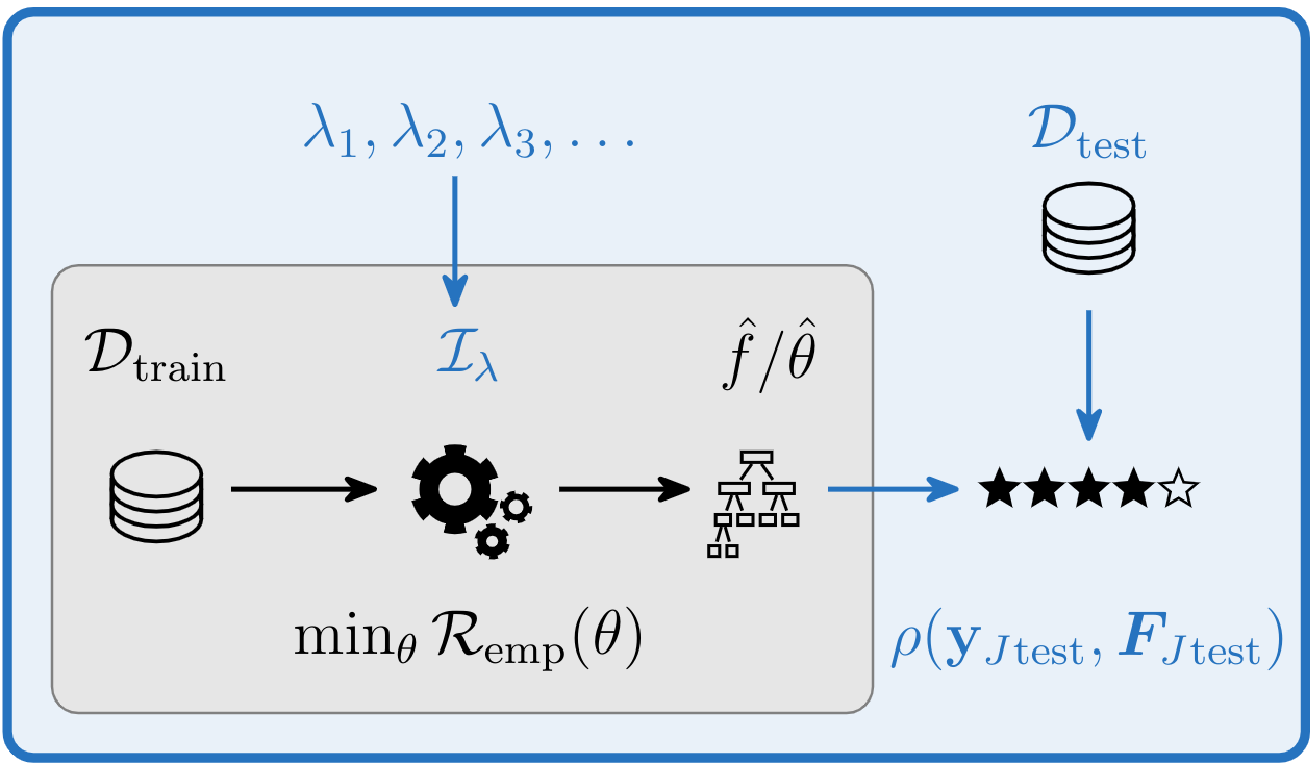
\includegraphics[width=0.8\textwidth]{figure_man/riskmin_bilevel3.png}
% \end{figure}
% \end{center}
% 
% \framebreak
%   \footnotesize
%   \begin{itemize}
%     \item For a learning algorithm $\inducer$ (also inducer) with $d$ hyperparameters, the hyperparameter \textbf{configuration space} is:
%       $$\Lam=\Lam_{1} \times \Lam_{2} \times \ldots \times \Lam_{d},$$
%       where $\Lam_{i}$ is the domain of the $i$-th hyperparameter.
%     \item The domains can be continuous, discrete or categorical.
%     \item For practical reasons, the domain of a continuous or integer-valued hyperparameter is typically bounded.
%     \item A vector in this configuration space is denoted as $\bm{\lambda} \in \Lam$.
%     \item A learning algorithm $\inducer$ takes a (training) dataset $\D \in \allDatasets$ and a hyperparameter configuration $\lamv \in \Lam$ and returns a trained model (through risk minimization)
% 
%     \vspace*{-0.2cm}
%   \begin{eqnarray*}
%     \inducer: \preimageInducer &\to& \Hspace \\
%     (\D, \lamv) &\mapsto& \inducer(\D, \lamv) = \hat f_{\D, \lamv}
%   \end{eqnarray*}
%     % \item Additionally, some hyperparameters may only need to be specified if another hyperparameter (or combination of hyperparameters) takes on a certain value.
%   \end{itemize}
% 
%   % \lz 
% 
%   % Note that 
% 
%   %   In contrast to the first-level (empirical) risk minimization problem, hyperparameter optimization is also referred to as \textbf{second-level} optimization. The first-level problem can be seen as a subroutine called by the second-level problem: Each evaluation of $\lamv$ requires to solve the first-level optimization problem.  
% 
% 
% %   \framebreak 
% 
% %   \begin{itemize}
% %     \item search for the \textbf{inducer} hyperparameter $\lamv$
% %     \item that minimizes the \textbf{generalization error}
% %       $$
% %         \min_{\lamv} \E_{\D_n \sim \Pxy, (\xv, y) \sim \Pxy} \left(V\left(y, \hat f_{\D, \lamv}(\xv)\right)\right). 
% %       $$
% %   \end{itemize}
% 
% % We compare: In empirical risk minimization, we 
%   
% %   \begin{itemize}
% %     \item search for the \textbf{model} parameter $\thetab$
% %     \item that minimizes the \textbf{empirical risk}
% %       $$
% %         \min_{\thetab} \sum_{(\xi, \yi) \in \Dtrain} L\left(\yi, \fxi\right). 
% %       $$
% %   \end{itemize}
% 
% %   In hyperparameter optimization, we
% 
% %   \begin{itemize}
% %     \item search for the \textbf{inducer} hyperparameter $\lamv$
% %     \item that minimizes the \textbf{test error}
% %       $$
% %         \min_{\lamv \in \Lam} \sum_{(\xi, \yi) \in \Dtest} V\left(\inducer(\Dtrain, \lamv)(\xi), \yi\right). 
% %       $$
% %   \end{itemize}
% 
% %   \framebreak 
% 
%     % \framebreak
%   
%   % The hyperparameter optimization problem is difficult in many ways: 
%   \end{vbframe}
% 
% 
% \begin{vbframe}{Tuning: A bi-level optimization problem} 
% We formally state the nested hyperparameter tuning problem as: 
% 
% $$
% \min_{\lamv \in \LamS} c(\lamv) \text{ where } c(\lamv) := \GEh_{\Dtrain, \Dtest}(\inducer,
%   \lamv, \ntrain, \rho)
% $$
% 
% \begin{itemize}
% \item The learner $\inducer(\Dtrain, \lamv)$ takes a training data set as well as hyperparameter settings $\lamv$ (e.g., the maximal depth of a classification tree) as an input. 
% \item The search space $\LamS$  is a bounded subset of $\Lam$.
% \item $\inducer(\Dtrain, \lamv)$ performs empirical risk minimization on the training data and returns the optimal model $\fh$ for the given hyperparameters. 
% \item Note that for the estimation of the generalization error, more sophisticated resampling strategies like cross-validation can be used.
% \end{itemize}
% 
% \framebreak

% The components of a tuning problem are: 

% \medskip
% We can thus define the HP tuner $\tau: (\D,\ind,\LamS,\rho)\mapsto \lamh$ that proposes its estimate $\lamh$ of the true optimal configuration $\lams$ given $\D, \Ilam$ with corresponding search space $\LamS$ to optimize, and a target measure $\rho$.

% \framebreak 

% \begin{center}
% \begin{figure}
% FIGURE SOURCE: https://docs.google.com/presentation/d/1JUtguuVBgidcqD0IdFFIiKH9zqYzM6YRjCqC53V90dA/edit?usp=sharing
% 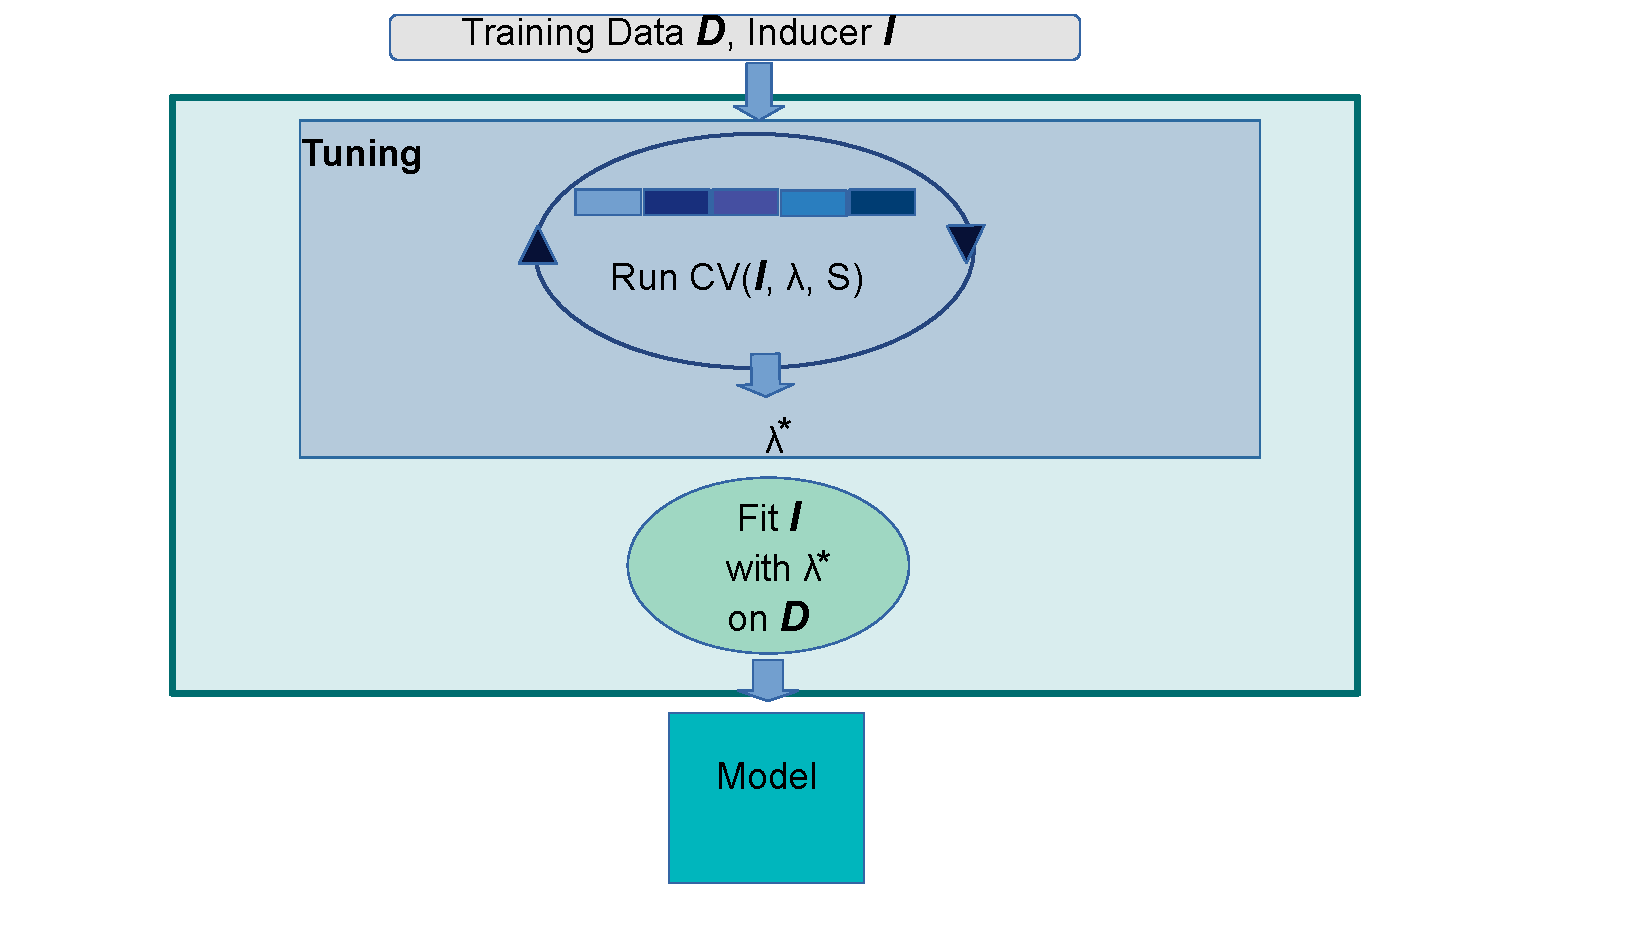
\includegraphics[width=1.2\textwidth]{figure_man/autotune_in_model_fit.pdf}
% \end{figure}
% \end{center}

% \end{vbframe}




% \framebreak

% Possible scenarios for finding default hyperparameters:

% \begin{itemize}
%   \item If the learner's performance is fairly insensitive to changes of a hyperparameter, we don't really have to worry as long as we remain within the range of reasonable values.
%   \item Constant default: we can benchmark the learner across a broad range of data sets and scenarios and try to find hyperparameter values that work well in many different situations. Quite optimistic?
%   \item Dynamic (heuristic) default: We can benchmark the learner across a broad range of data sets and scenarios and try to find an easily computable function that sets the hyperparameter in a data dependent way,
%   e.g. using \texttt{mtry}$ = p/3$ for RF.\\
%     How to construct or learn that heuristic function, though...?
%   \item In some cases, can try to set hyperparameters optimally by extracting more info from the fitted model. E.g. \texttt{ntrees} for a random forest (does OOB error increase or decrease if you remove trees from the ensemble?).
% \end{itemize}
% \end{vbframe}


\begin{vbframe}{Why is tuning so hard?}
  \begin{itemize}
\item Tuning is usually \textbf{black box}: No derivatives of the objective are availabe. 
    We can only eval the performance for a given HPC via a computer program (CV of learner on data).
\item Every evaluation can require multiple train and predict steps, hence it's \textbf{expensive}.
\item Even worse: the answer we get from that evaluation is \textbf{not exact, but stochastic} in most settings, as we use resampling.
\item \textbf{Categorical and dependent hyperparameters} aggravate our difficulties: the space of hyperparameters we optimize over can have non-metric, complicated structure.
\item Many standard optimization algorithms cannot handle these properties.
\end{itemize}

  \end{vbframe}

\endlecture

\end{document}
